\documentclass[9pt,twocolumn,twoside]{osajnl}

\journal{ol} % Choose journal (ao, aop, josaa, josab, ol)
\usepackage{amsmath}

% See template introduction for guidance on setting shortarticle option
\setboolean{shortarticle}{false} 
% true = letter / tutorial 
% false = research / review article 
% (depending on journal).


\title{Experiment 5: The Stirling Cycle}

\author[1]{Nathaniel Comeau, V00856678}

\affil[1]{Physics Department, University of Victoria}

%% To be edited by editor
% \dates{Compiled \today}

\ociscodes{}

%% To be edited by editor
% 

\begin{abstract}
The thermodynamic work done by a Stirling Engine was determined to be 2185.6 Joules. The power generated by the engine was determined to be 10.62kW. The efficiency rating $\eta$ was found to be 0.015.
\end{abstract}

\setboolean{displaycopyright}{false}

\begin{document}

\maketitle

\section{Introduction}
The Stirling engine is a heat engine with a high-efficiency rating of up to 50\%\cite{stirling50}. Stirling engines are compatible with some renewable energy sources and may become increasingly important as fuel costs rise\cite{stirlingwiki}. Hence a basic understanding of the Stirling and Carnot heat-engine cycles is important.

\section{Theory}
\label{sec:theory}

The ideal Stirling engine cycle is made up of two isothermal and two isochoric sections. Figure 1 demonstrates the relevant portions\cite{stirlingdiagram}.%Mention working fluid

\begin{figure}[htbp]
\centering
\fbox{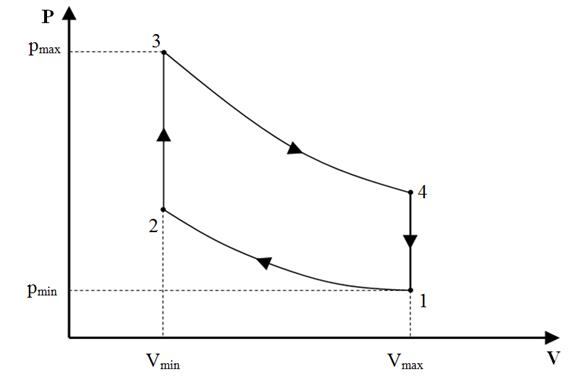
\includegraphics[width=\linewidth]{stirlingcycle}}
\caption{Stirling Cycle. Note the two isothermal and two isochoric sections.}
\label{fig:stirlingcycle}
\end{figure}
Sections 12 is an isothermal compression of the working fluid. Section 23 demonstrated isochoric heating of the fluid. Section 34 is an isothermal expansion and section 41 demonstrates isochoric cooling.

One of the most important applications of the Stirling cycle is the Stirling engine.\cite{labmanual} A Beta Stirling engine uses a displacement and power piston mounted in the same cylinder to convert heat energy to mechanical work.\cite{stirlingwiki} Figure 2 demonstrates an implementation of the theoretical Strirling Cycle.

\begin{figure}[htbp]
\centering
\fbox{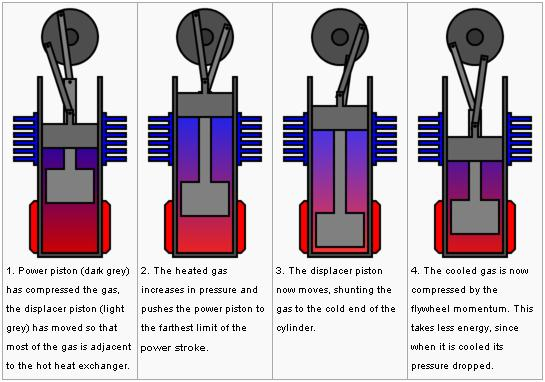
\includegraphics[width=\linewidth]{betastirlingcycle}}
\caption{Beta Stirling engine implementation of Stirling Cycle.}
\label{fig:stirlingcycle}
\end{figure}
Once the engine has been started the efficiency can be obtained by 
\begin{equation} \label{efficiency}
\eta = \frac{P_1}{P_2}
\end{equation}
where $P_1$ is the power output and $P_2$ is the power input.

If a braking force F is applied to the flywheel spindle then \(P_{out} = P_1 = F\cdot2\pi f\cdot r\) where $r$ is the spindle radius and $f$ is the frequency in cycles/second. The input power is from the heated coil and hence 
\begin{equation} \label{pout}
P_{out} = P_2 = IV = I^2R
\end{equation}
where $I$ is the coil current and $V$ is the voltage across the coil.\cite{labmanual}

\section{Experimental Procedure}

By tracking the displacement of the working piston and the cylinder internal pressure $P$ and $V$ can be simultaneously plotted to produce a $PV$ plot. The sensor voltages are first calibrated. The engine was then started by the procedure in the lab manual.\cite{labmanual} Five runs of data were recorded. The period under no load was recorded. 

\begin{figure}[htbp]
\centering
\fbox{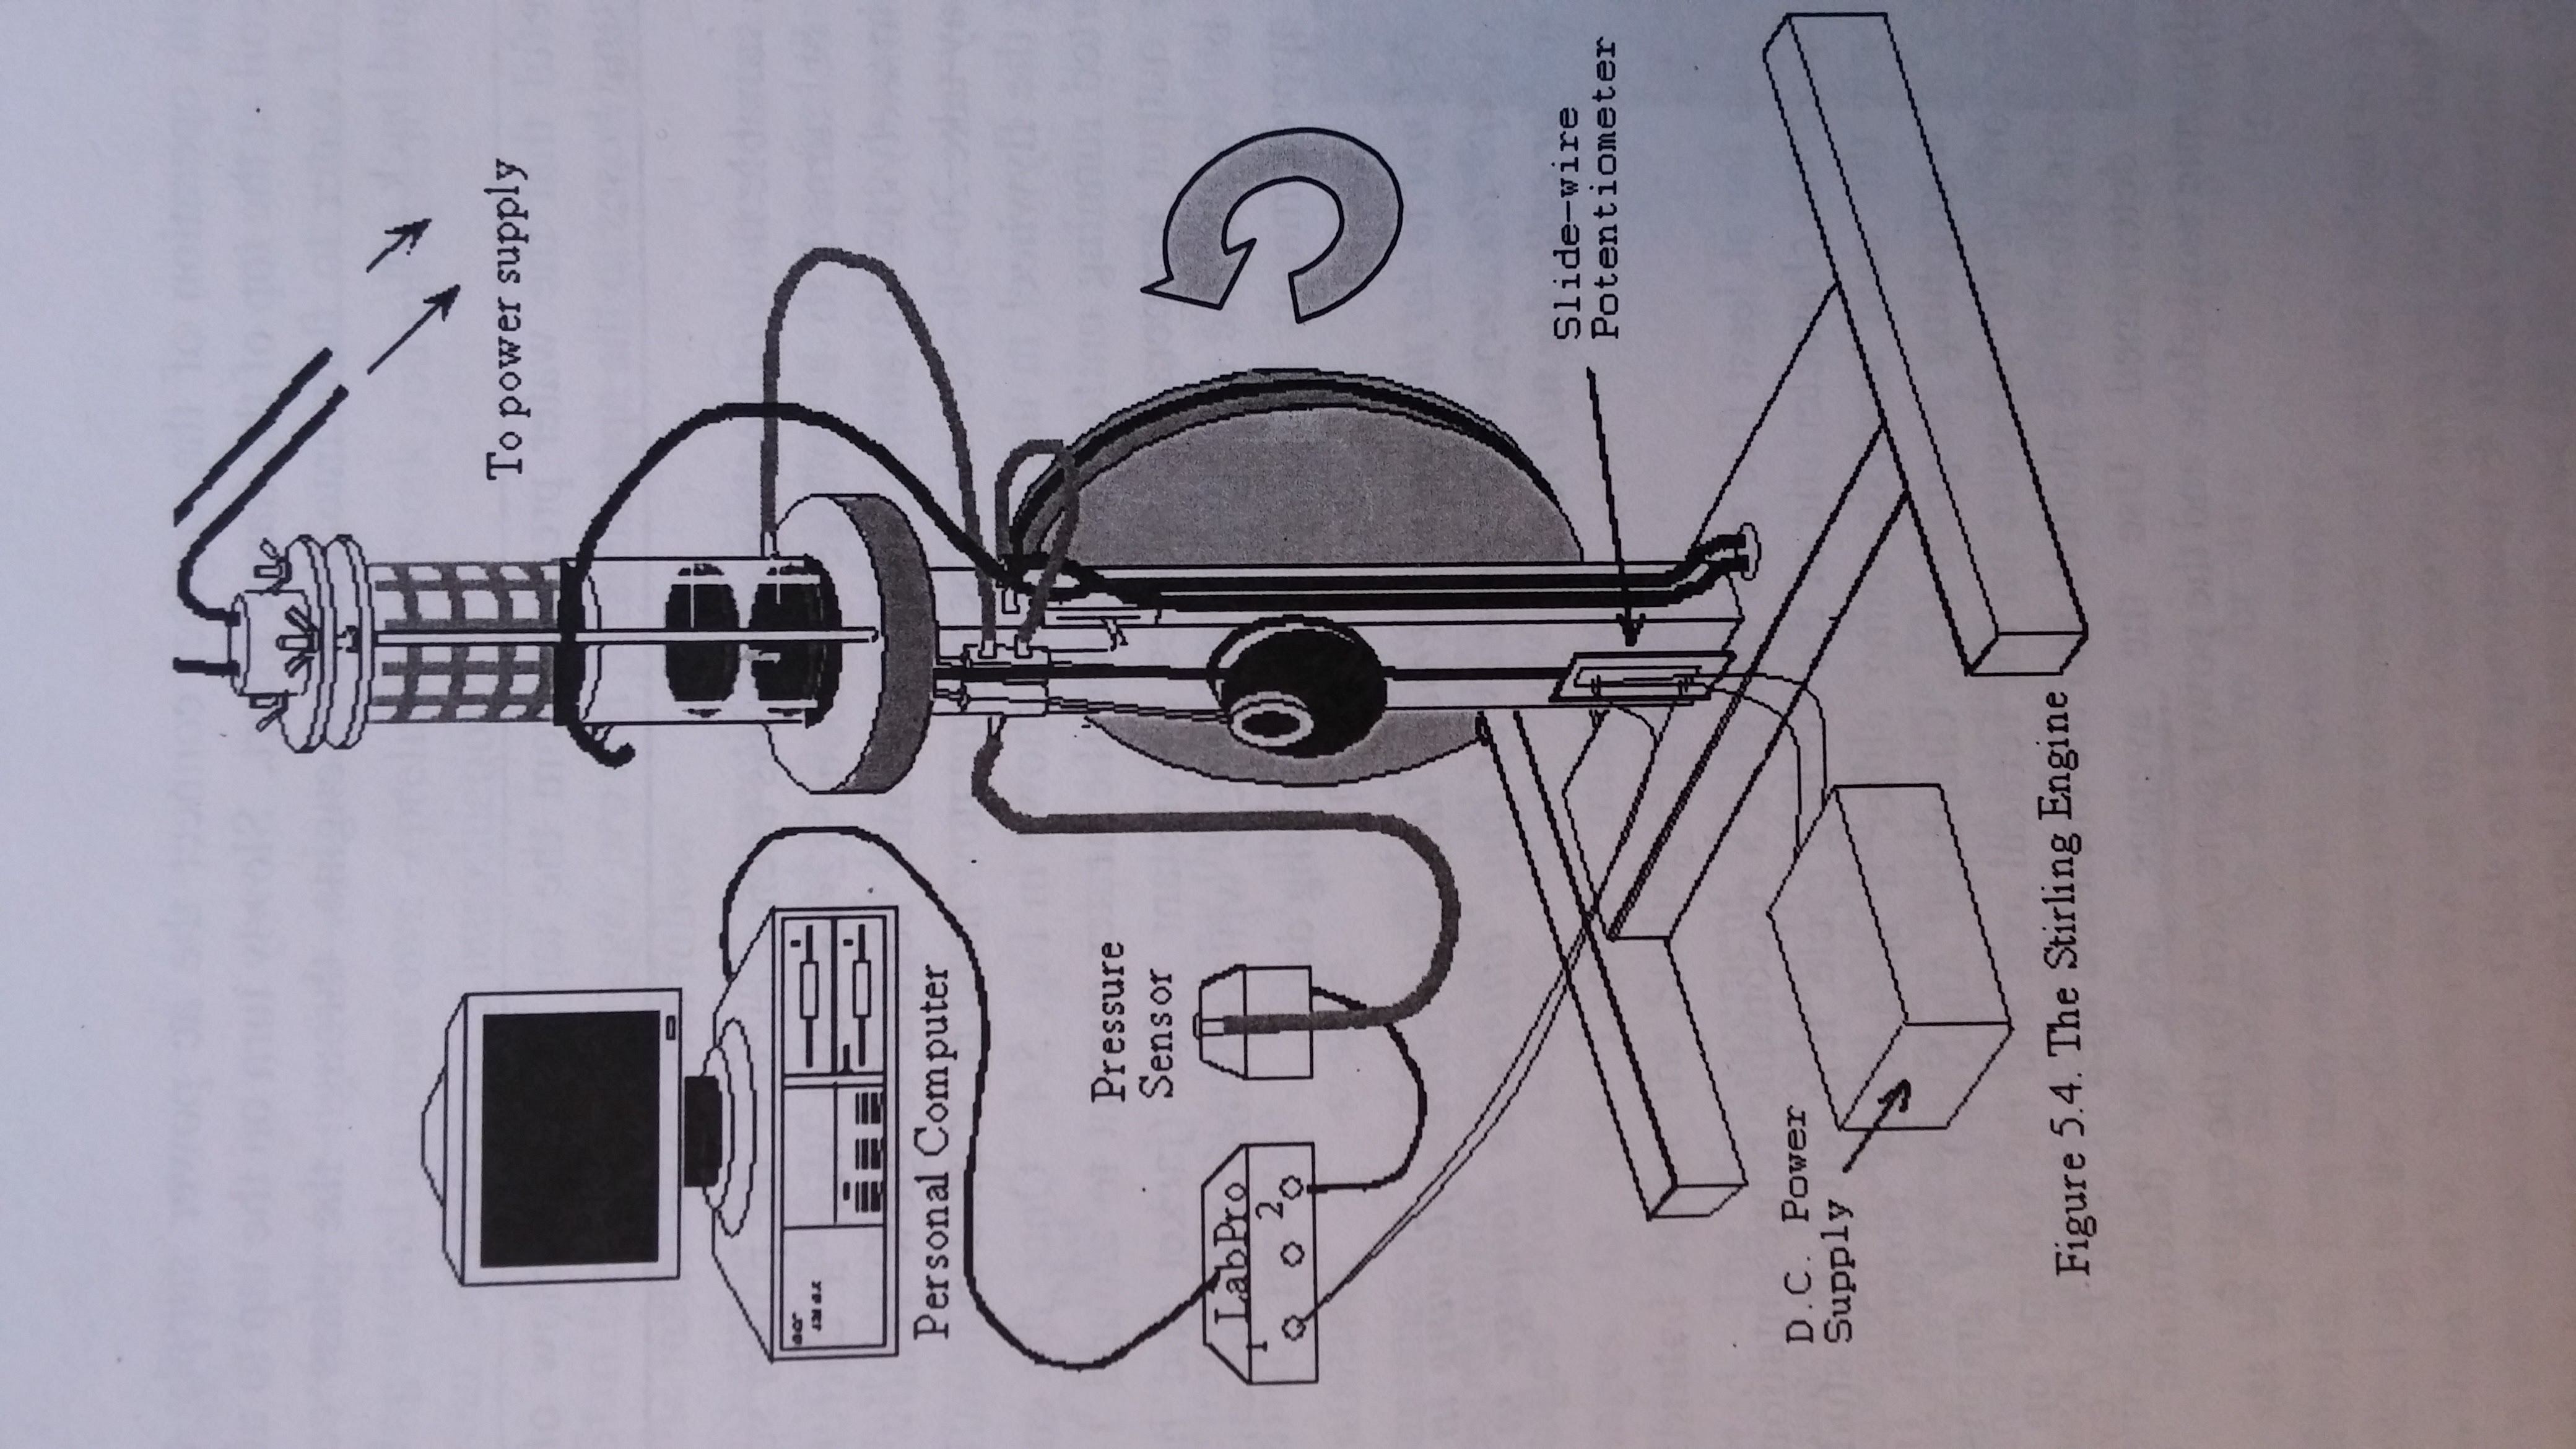
\includegraphics[width=\linewidth,angle=-90,origin=c]{exp5diagram}}
\caption{Beta Stirling engine and experimental apparatus used in the experiment.}
\label{fig:experimentdiagram}
\end{figure}

The engine was then slowed down by wrapping a braided copper band around the spindle of the flywheel. The frequency of the engine under load, the spring scale readings and the radius of the spindle was recorded.

\section{Discussion of Results}

Figure 3 %This the physical integral you printed off.
demonstrates a captured $PV$ curve. 
\subsection{Question1}
The integral of this curve is in units \[kPa\cdot cm^3 = \frac{kg}{m\cdot s^2}\cdot m^3 = kg\cdot m^2 s^{-2} = Joules\] which is shown by dimensional analysis to be the thermodynamic work done by the engine. 

The average area (see table 1) was determined to be 2185.6; thus the thermodynamic work done was 2185.6 Joules. Because from the measured period $T_{noload} =0.206$ and $f =4.86s^{-1}$, %Have to include period calculation and data figure.!
\[P_{generated} = Work\cdot f = 2185.6J\cdot 4.86s^-1 = 10.62kW\]

Comparing the obtained PV curve Figure 3 to the ideal curve Figure 1 shows a lack of the two vertical isochoric sections. Instead two isothermal curves similar to a Carnot cycle seem to intersect. 

The efficiency of the engine can be calculated from equation 1 as \[\eta = \frac{3.0N\cdot 2\pi 4.86s^-1\cdot 0.0253m}{(12.00\pm0.05A)^2\cdot 1.04\Omega\pm0.4\%} = 0.015\]
Note that $P_{out} = 2.3W$ from this expression.
This low efficiency rating shows sources of thermal energy loss. 

One source of energy loss is waste heat passed to the environment by the cooling water and heat sink. Any radiated to the environment that does not go into mechanical energy is waste. Another smaller source of thermal energy loss is radiation through the cylinder walls before reaching the heat sink.

\subsection{Question two}

Equation 5.2 states that
\begin{equation}
P_1 = F\cdot2\pi f\cdot r
\end{equation}
Recall that rotational power can be defined as
\begin{equation}
P = \frac{dW}{dT} = \tau \frac{d\theta}{dt} = \tau2\pi f
\end{equation}
which is equivalent to
\begin{equation}
P = F\cdot \vec{r} \cdot sin\theta  2\pi f
\end{equation}
where \(sin\theta = 1\) because the considered force is perpendicular to $\vec{r}$ at every point.\cite{rotationalpower}

Figure 4 shows a braking force perpendicular to the counter-clockwise rotation of the engine.
\begin{figure}[htbp]
\centering
\fbox{\includegraphics[width=\linewidth]{ForceDiagram}}
\caption{Force diagram demonstrating applied forces.}
\label{fig:forcediagram}
\end{figure}

\bigskip

% Bibliography


% Full bibliography added automatically for Optics Letters submissions; the following line will simply be ignored if submitting to other journals.
% Note that this extra page will not count against page length
 
%anual citation list
\begin{thebibliography}{1}
\bibitem{labmanual}
Phys 217 Lab Manual
\bibitem{rotationalpower}
\url{http://www.engineeringtoolbox.com/angular-velocity-acceleration-power-torque-d_1397.html}
\bibitem{stirling50}
\url{http://www.mpoweruk.com/stirling_engine.htm}
\bibitem{stirlingwiki}
\url{https://en.wikipedia.org/wiki/Stirling_engine}
\bibitem{stirlingdiagram}
\url{http://ibimapublishing.com/uploads/926227-fig-1.jpg}
\bibitem{betastirlingcycle}
\url{https://s-media-cache-ak0.pinimg.com/originals/23/25/e3/2325e39b7b04ef88a08ab9db1e3b188c.jpg}

\end{thebibliography}
\bigskip
\section{Appendix}
\subsection{data}

\begin{table}[htbp]
\centering
\caption{\bf Area of five runs}
\begin{tabular}{ccc}
\hline
run & area (J) \\
\hline
1 & 2158\\
2 & 2343\\
3 & 2093\\
4 & 2144\\
5 & 2190\\
\hline
average & 2185.6\\

\hline
\end{tabular}
  \label{tab:shape-functions}
\end{table}

\end{document}
